\documentclass[12pt]{article}
\usepackage[margin=1in]{geometry}
\usepackage{amsmath}
\usepackage{enumitem}
\usepackage{xcolor}
\usepackage{mathtools}
\usepackage{amssymb, amsthm}
\usepackage{tikz}
\usepackage{tkz-graph}
\usepackage{multicol}
\usetikzlibrary{arrows,automata}
\usepackage[nointegrals]{wasysym}
\newcommand{\red}[1]{\textcolor{red}{#1}}

\begin{document}
\title{MA-236: Homework 12}
\author{Rob Herley}
\maketitle

\begin{center}
I pledge my honor that I have abided by the Stevens Honor System.
\end{center}

\begin{center}
  "Prove that $0 \times ss0 = 0$ in Robinson arithmetic."
\end{center}

\noindent
Pruned Tree where $Q_1...Q_7$ are the axioms of Robinson's arithmetic:

\begin{center}
  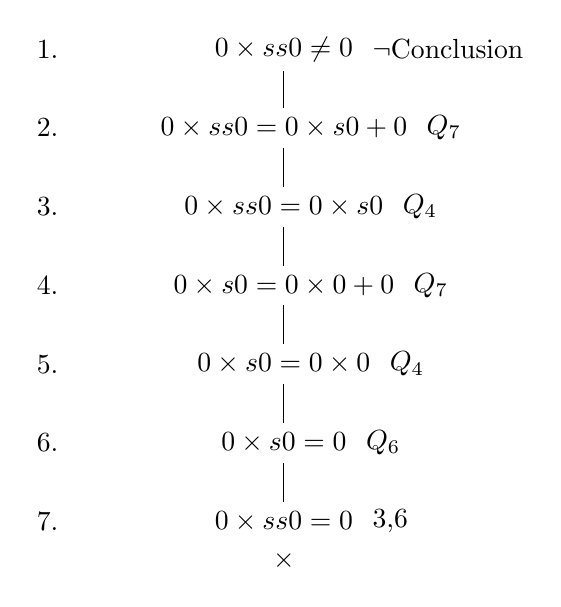
\begin{tikzpicture}
  \draw (-1cm,0)      node (11)                       {1.};
  \draw (2cm,0)    node (13) [label=right:$\neg$Conclusion] {$0 \times ss0 \neq 0$};
  
  \draw (-1cm,-1cm)   node (21)                      {2.};
  \draw (2cm,-1cm) node (23) [label=right:$Q_7$] {$0 \times ss0 = 0 \times s0 + 0$};
  \draw (13) -- (23);
  
  \draw (-1cm,-2cm)   node (31)                      {3.};
  \draw (2cm,-2cm) node (33) [label=right:$Q_4$] {$0 \times ss0 = 0 \times s0$};
  \draw (23) -- (33);
  
  \draw (-1cm,-3cm)   node (41)                      {4.};
  \draw (2cm,-3cm) node (43) [label=right:{$Q_7$}]{$0 \times s0 = 0 \times 0 + 0$};
  \draw (33) -- (43);

  \draw (-1cm,-4cm)   node (51)                      {5.};
  \draw (2cm,-4cm) node (53) [label=right:{$Q_4$}]{$0 \times s0 = 0 \times 0$};
  \draw (43) -- (53);

  \draw (-1cm,-5cm)   node (61)                      {6.};
  \draw (2cm,-5cm) node (63) [label=right:{$Q_6$}]{$0 \times s0 = 0$};
  \draw (53) -- (63);

  \draw (-1cm,-6cm)   node (71)                      {7.};
  \draw (2cm,-6cm) node (73) [label=right:{$3$,$6$}][label=below:{$\times$}]{$0 \times ss0 = 0$};
  \draw (63) -- (73);

  
  \end{tikzpicture}
  \end{center}

\noindent
Since the pruned refutation tree closes, the sentences are \textbf{inconsistent}.
Therefore, the argument is \textbf{valid}.

\end{document}

